\documentclass[a4paper, 11pt]{article}

\usepackage[czech]{babel}
\usepackage[utf8]{inputenc}
\usepackage[left=2cm, top=3cm, text={17cm, 24cm}]{geometry}
\usepackage{times}
\usepackage{multirow}
\usepackage[ruled, czech, linesnumbered, noline, longend]{algorithm2e}
\usepackage{graphics}
\usepackage{pdflscape}
\begin{document}
\makeatletter
\begin{titlepage}
	\begin{center}
		{\Huge \textsc{Vysoké učení technické v Brně}} \\[0.5em]
		{\huge \textsc{Fakulta informačních technologií}} \\[0.6em]
		\vspace{\stretch{0.382}}
		\quad\hbox{\LARGE{Typografie a publikování -- 3. projekt}} \\[0.6em]
		\quad\hbox{\Huge{Tabulky a obrázky}}
		\vspace{\stretch{0.618}}
	\end{center}
	\begin{flushright}
		{\Large \today} \hfill {\Large Josef Pasek}
	\end{flushright}
\end{titlepage}
\makeatother
\section{Úvodni strana}

Název práce umístěte do zlatého řezu a nezapomeňte uvést \textit{dnešní} (today) datum a vaše jméno a příjmení.

\section{Tabulky}

Pro sázení tabulek můžeme použít buď prostředí\texttt{ tabbing }nebo prostředí\texttt{ tabular}.
\subsection{Prostředí \texttt{ tabbing}}

Při použití tabbing vypadá tabulka následovně:

\begin{tabbing}
	Ovoce \hspace{1.5cm} \= Množství \hspace{0.3cm} \= Jednotka \hspace{0.3cm} \= Cena za jedn. \hspace{0.3cm} \= Cena celková \kill
	\textbf{Ovoce} \> \textbf{Množství} \> \textbf{Jednotka} \> \textbf{Cena za jedn.} \> \textbf{Cena celková} \\
	Jablka \> 3 \> kg \> 25,90 Kč \> 77,70 Kč \\
	Hrušky \> 2,5 \> kg \> 27,40 Kč \> 68,50 Kč \\
	Vodní melouny \> 1 \> kus \> 35,--Kč \> 35,--Kč \\
\end{tabbing}
Toto prostředí se dá také použít pro sázení algoritmů, ovšem vhodnější je použít
prostředí\texttt{ algorithm }nebo\texttt{ algorithm2e }(viz sekce~\ref{section:algoritmy}).
\subsection{Prostředí tabular}
Další možností, jak vytvořit tabulku, je použít prostředí\texttt{ tabular}. Tabulky pak
budou vypadat takto\footnotemark:

\bigskip
\begin{table}[h]
	\catcode`\-=12
	\centering
	\begin{tabular}{|c|c|c|}
		\hline
		~             & \multicolumn{2}{c|}{\textbf{Cena}}                   \\
		\cline{2-3}
		\textbf{Měna} & \textbf{nákup}                     & \textbf{prodej} \\
		\hline
		EUR           & 23,26                              & 24,93           \\
		GBP           & 29,56                              & 29,86           \\
		USD           & 22,27                              & 23              \\
		\hline
	\end{tabular}
	\caption{Tabulka kurzů k~dnešnímu dni}
	\label{table:kurzy}
\end{table}
\bigskip
\begin{table}[h]
	\centering
	\catcode`\-=12
	\begin{tabular}{|c|c|}
		\hline
		\multicolumn{1}{|c|}{A} & $\neg A$ \\
		\hline
		P                       & N        \\
		\hline
		O                       & O        \\
		\hline
		X                       & X        \\
		\hline
		N                       & P        \\
		\hline
	\end{tabular}
	\begin{tabular}{|c|c|c|c|c|c|}
		\hline
		\multicolumn{2}{|c|}{\multirow{2}{*}{A $\land$ B}} & \multicolumn{4}{c|}{B}                                            \\ \cline{3-6}
		\multicolumn{2}{|c|}{}                             & \textbf{P}             & \textbf{O} & \textbf{X} & \textbf{N}     \\ \hline
		\multirow{4}{*}{A}                                 & \textbf{P}             & P          & O          & X          & N \\ \cline{2-6}
		                                                   & \textbf{O}             & O          & O          & N          & N \\ \cline{2-6}
		                                                   & \textbf{X}             & X          & N          & X          & N \\ \cline{2-6}
		                                                   & \textbf{N}             & N          & N          & N          & N \\ \hline
	\end{tabular}
	\begin{tabular}{|c|c|c|c|c|c|}
		\hline
		\multicolumn{2}{|c|}{\multirow{2}{*}{A $\lor$ B}} & \multicolumn{4}{c|}{B}                                            \\ \cline{3-6}
		\multicolumn{2}{|c|}{}                            & \textbf{P}             & \textbf{O} & \textbf{X} & \textbf{N}     \\ \hline
		\multirow{4}{*}{A}                                & \textbf{P}             & P          & O          & X          & N \\ \cline{2-6}
		                                                  & \textbf{O}             & O          & O          & N          & N \\ \cline{2-6}
		                                                  & \textbf{X}             & X          & N          & X          & N \\ \cline{2-6}
		                                                  & \textbf{N}             & N          & N          & N          & N \\ \hline
	\end{tabular}
	\begin{tabular}{|c|c|c|c|c|c|}
		\hline
		\multicolumn{2}{|c|}{\multirow{2}{*}{A $\rightarrow$ B}} & \multicolumn{4}{c|}{B}                                            \\ \cline{3-6}
		\multicolumn{2}{|c|}{}                                   & \textbf{P}             & \textbf{O} & \textbf{X} & \textbf{N}     \\ \hline
		\multirow{4}{*}{A}                                       & \textbf{P}             & P          & O          & X          & N \\ \cline{2-6}
		                                                         & \textbf{O}             & O          & O          & N          & N \\ \cline{2-6}
		                                                         & \textbf{X}             & X          & N          & X          & N \\ \cline{2-6}
		                                                         & \textbf{N}             & N          & N          & N          & N \\ \hline
	\end{tabular}
	\caption{
		Protože Kleeneho trojhodnotová logika už je \uv{zastaralá}, uvádíme si zde
		příklad čtyřhodnotové logiky
	}
	\label{table:logika}
\end{table}
\bigskip
\footnotetext{
	Kdyby byl problem s\texttt{ cline,} zkuste se podívat třeba sem:
	http://www.abclinuxu.cz/tex/poradna/show/325037.
}
\pagebreak
\section{Algoritmy}\label{section:algoritmy}
Pokud budeme chtít vysázet algoritmus, můžeme použít prostředí\texttt{ algorithm\footnote{
		Pro nápovědu, jak zacházet s~prostředím\texttt{ algorithm,} můžeme zkusit tuhle stránku: \\
		http://ftp.cstug.cz/pub/tex/CTAN/macros/latex/contrib/algorithms/algorithms.pdf.
	} }
nebo\texttt{ algorithm2e\footnote{
		Pro\texttt{ algorithm2e }zase tuhle:
		http://ftp.cstug.cz/pub/tex/CTAN/macros/latex/contrib/algorithm2e/doc/algorithm2e.pdf.
	}}. Příklad použití prostředí\texttt{ algorithm2e }viz Algoritmus~\ref{algorithm:fastslam}. \\
\IncMargin{1.5em}

\begin{algorithm}
	\caption{\textsc{FastSLAM}}
	\label{algorithm:fastslam}

	\SetNlSty{}{}{:}
	\SetNlSkip{0.4emp}
	\SetAlgoNlRelativeSize{-1}
	\SetInd{1em}{1em}

	\Indm\Indmm
	\KwIn{$ (X_{t - 1}, u_t, z_t) $}
	\KwOut{$ X_t $}
	\Indp\Indpp
	\BlankLine

	$\overline{X_t} = X_t = 0$ \\

	\For{$ k = 1 \textrm{\emph{ to }} M $}{
	$(x_t)^{[k]} = \emph{sample\_motion\_model}(u_t,(x_{t-1})^{[k]}$ \\
	$(\omega_t)^{[k]} = \emph{measurement\_model}(z_t,(x_{t-1})^{[k]},m_{t-1}$) \\
	$(m_t)^{[k]} = \emph{updated\_occupancy\_grid}(z_t,(x_{t-1})^{[k]},(m_{t-1})^{[k]}$) \\
	$ \overline{X_t} = \overline{X_t} + \langle x_x^{[m]}, \omega_t^{[m]}  \rangle $ \\
	}
	\For{$ k = 1 \textrm{\emph{ to }} M $}{
	draw $ i $ with probability $\approx \omega_{t}^{[i]}$ \\
	add $\langle x_x^{[k]},m_t^{[k]} \rangle X_t$
	}
\end{algorithm}
\section{Obrázky}
Do našich článků můžeme samozřejmě vkládat obrázky. Pokud je obrázkem fotografie, můžeme klidně použít
bitmapový soubor. Pokud by to ale mělo být nějaké schéma nebo něco podobného, je dobrým zvykem takovýto
obrázek vytvořit vektorově.
\reflectbox{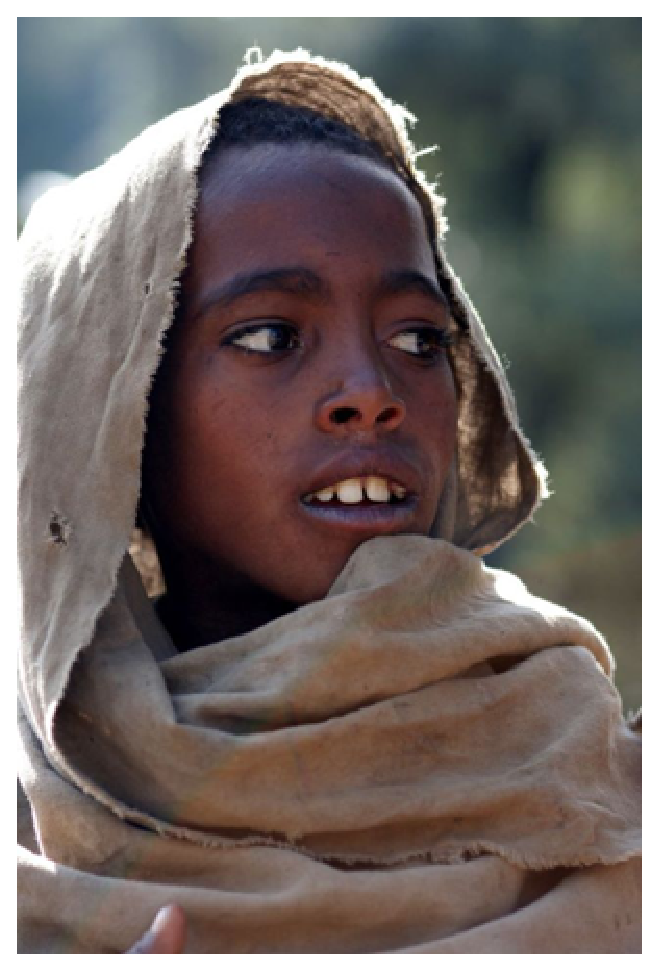
\includegraphics{/home/tjoslef/skola/vut/zapisky_vut/ITY/projekt3/etiopan.eps}}
\end{document}
